\section*{Assignment 08: Metrics and Learning}
\addcontentsline{toc}{section}{Assignment 08: Metrics and Learning}

This assignment summarises the handful of metrics we actually use so SkillSync decisions lean on evidence rather than hunches.

\subsection*{KPIs that make sense}
\begin{itemize}
    \item \textbf{Matching rate}: Share of suggested matches accepted; when it drops we tweak onboarding questions or algorithm weights.
    \item \textbf{Repeat usage}: Users returning within 30 days; a dip means retention nudges or community events need work.
    \item \textbf{NPS}: Early signal of fairness or stability issues, paired with quick interviews.
    \item \textbf{Time-to-first-value}: Minutes to the first meaningful action; friction in onboarding shows up here.
    \item \textbf{Revenue per active match}: Confirms monetisation scales with engagement rather than a few whales.
    \item \textbf{Equity of participation}: Tracks how many projects come from resource-light partners so inclusion stays visible.
\end{itemize}

\subsection*{Data infrastructure and feedback loop}
Events land in a cloud warehouse via Segment-style pipelines, dbt shapes usable tables, and shared dashboards in Looker Studio or Metabase keep the team in sync. We run three review cadences: weekly triage of anomalies, monthly cohort analyses by acquisition channel, and quarterly learning readouts that reset hypotheses while keeping the informal student vibe.

\subsection*{How metrics guide change}
When the matching rate fell from 62\% to 48\% for a partner cohort we tightened onboarding questions, rebalanced weights, and within two sprints the metric climbed back above 60\%, repeat usage rebounded, and revenue per match stabilised. Because we also watch equity of participation we confirmed NGO supply stayed healthy, so the fix helped both sides.

Figure~\ref{fig:feedback-screen} shows the light-touch feedback form that feeds those dashboards: a three-tap rating, a short note, and impact badges that reward good collaboration. Scores feed the matching model while flagged notes head to moderators.

\begin{figure}[h]
  \centering
  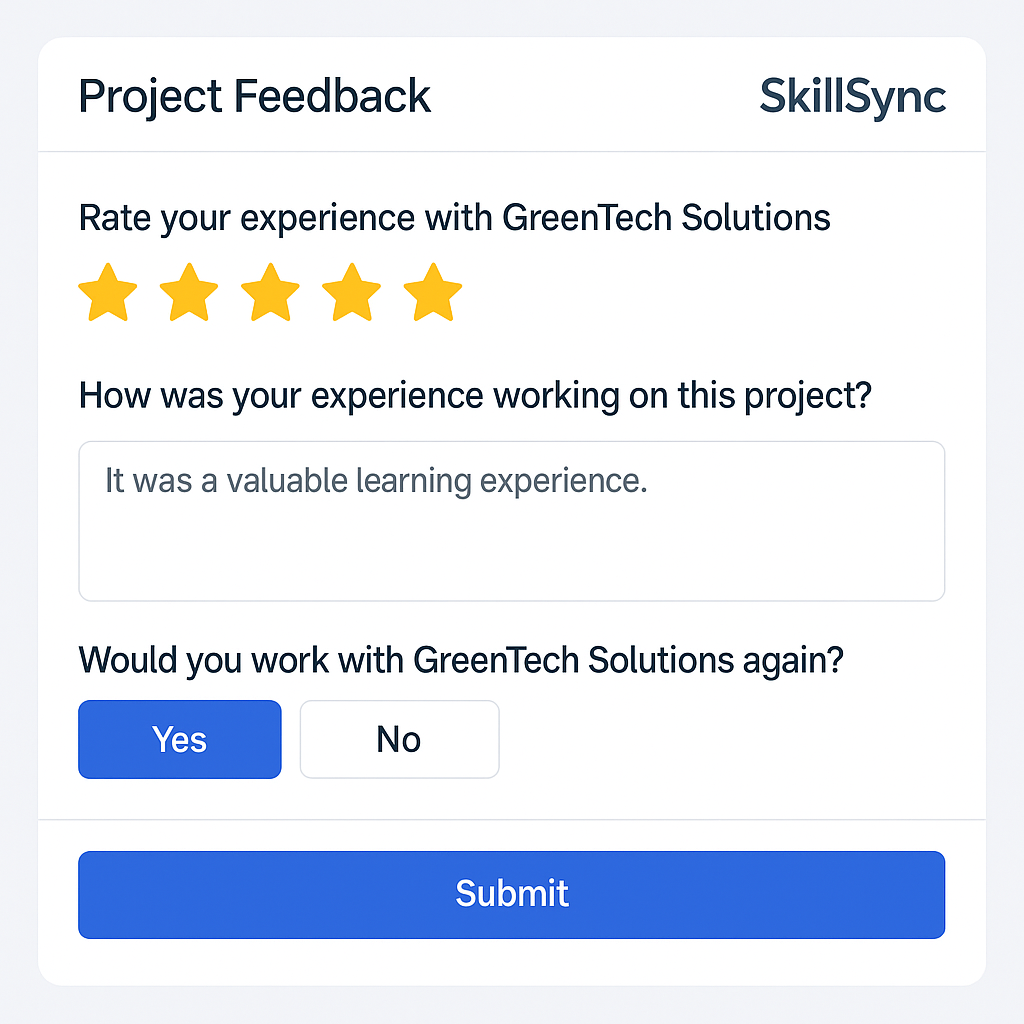
\includegraphics[width=0.8\linewidth]{figures/opgave08/feedback-vurderingsskaerm.png}
  \caption{Feedback and evaluation screen (`feedback-vurderingsskaerm.png`) that powers the KPI loop.}
  \label{fig:feedback-screen}
\end{figure}

We lock the definitions down with tooltips linking back to dbt models, version-control the SQL, and archive quarterly snapshots of the KPI board. Those mundane rituals turn metrics into institutional memory, echoing \citet{Choudary2016}'s push to institutionalise learning.
